% sharp.tex

\section{Mach 3 flow over a sharp-nosed two-dimensional body}
%
The specifications for this example come from section 5.2
in JD Anderson's Hypersonics book \cite{anderson_89}.
It shows the use of a \texttt{spline} curve as well as being a source
of test data for the Method-of-Characteristics for rotational flow.
Data for the spline points was computed from
$$
\frac{y}{y_e} = -0.008333 + 0.609425 \left( \frac{x}{y_e} \right)
                - 0.092593 \left( \frac{x}{y_e} \right)^2
$$
where $y_e = 1.0$.

\begin{figure}[htbp]
\begin{center}
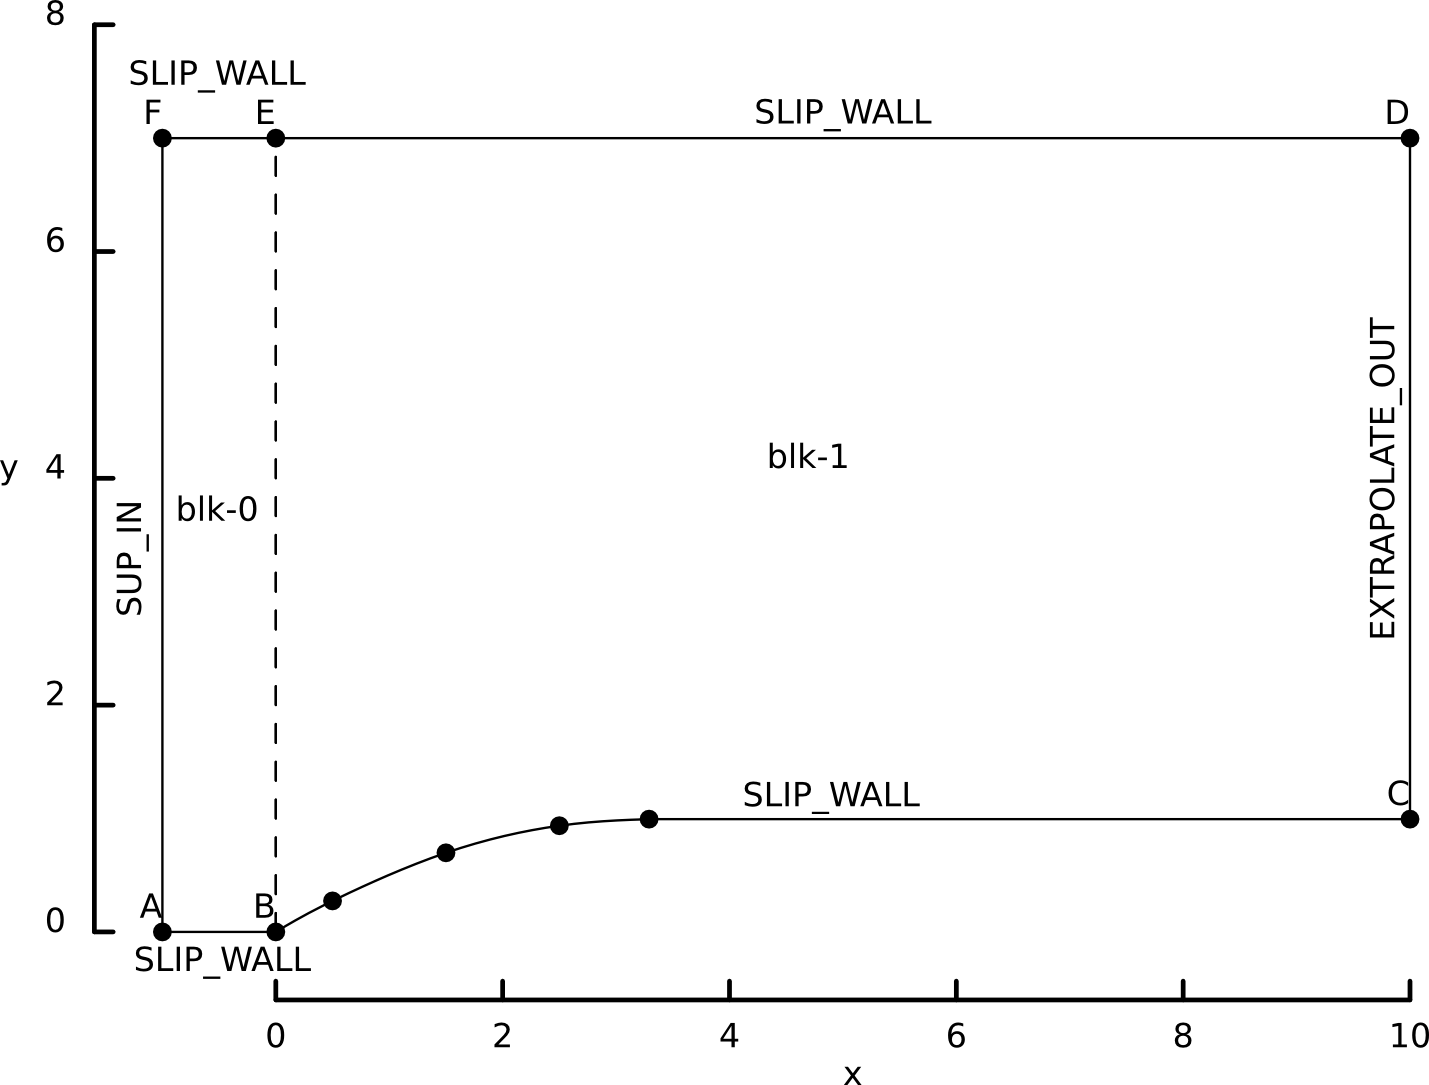
\includegraphics[width=12cm]{../2D/sharp/sharp.png}
\end{center}
\caption{Schematic diagram of the geometry for the sharp body.}
\label{sharp-geometry-fig}
\end{figure}

\begin{figure}[htbp]
\begin{center}
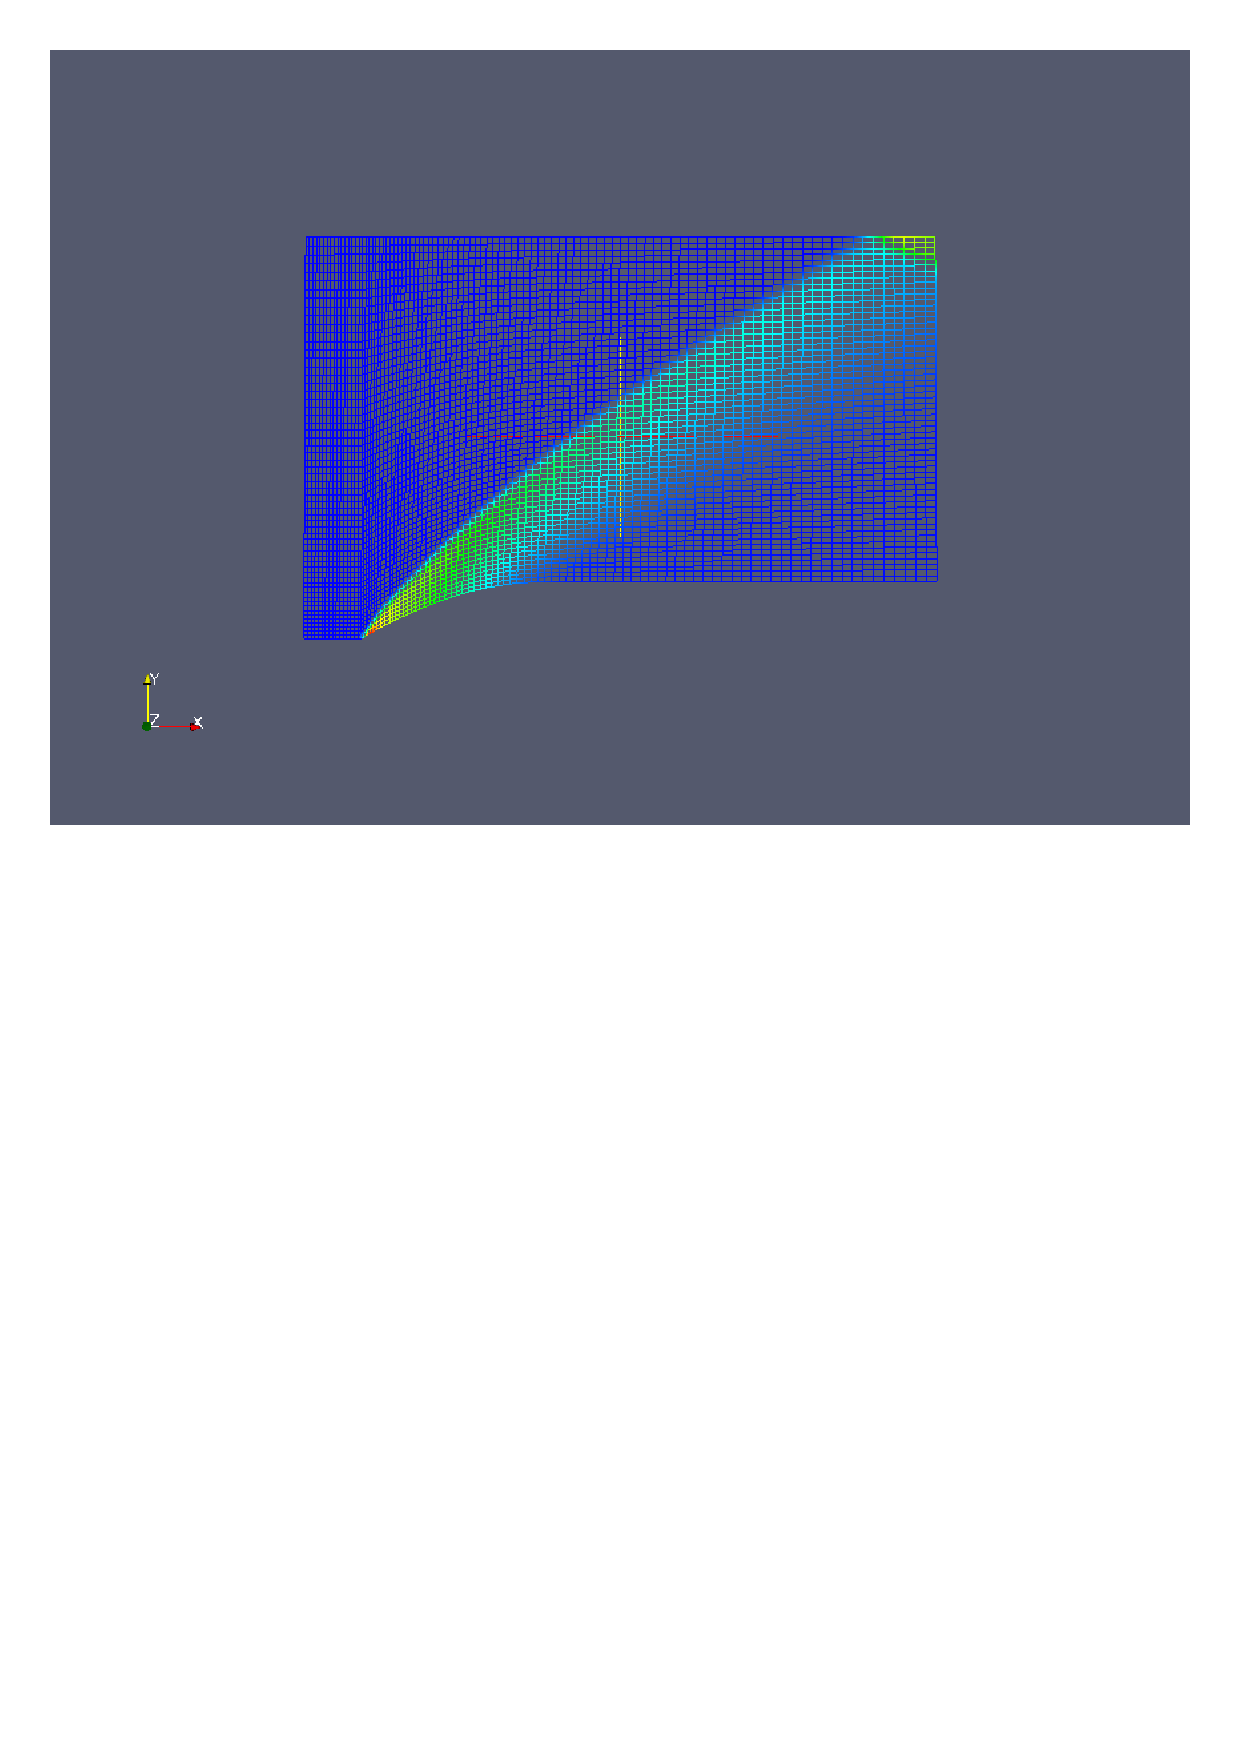
\includegraphics[width=\textwidth, viewport=24 446 570 818]{../2D/sharp/sharp_mesh.pdf}
\end{center}
\caption{Mesh, coloured by pressure, for the sharp body exercise.}
\label{sharp-mesh-fig}
\end{figure}

\begin{figure}[htbp]
\begin{center}
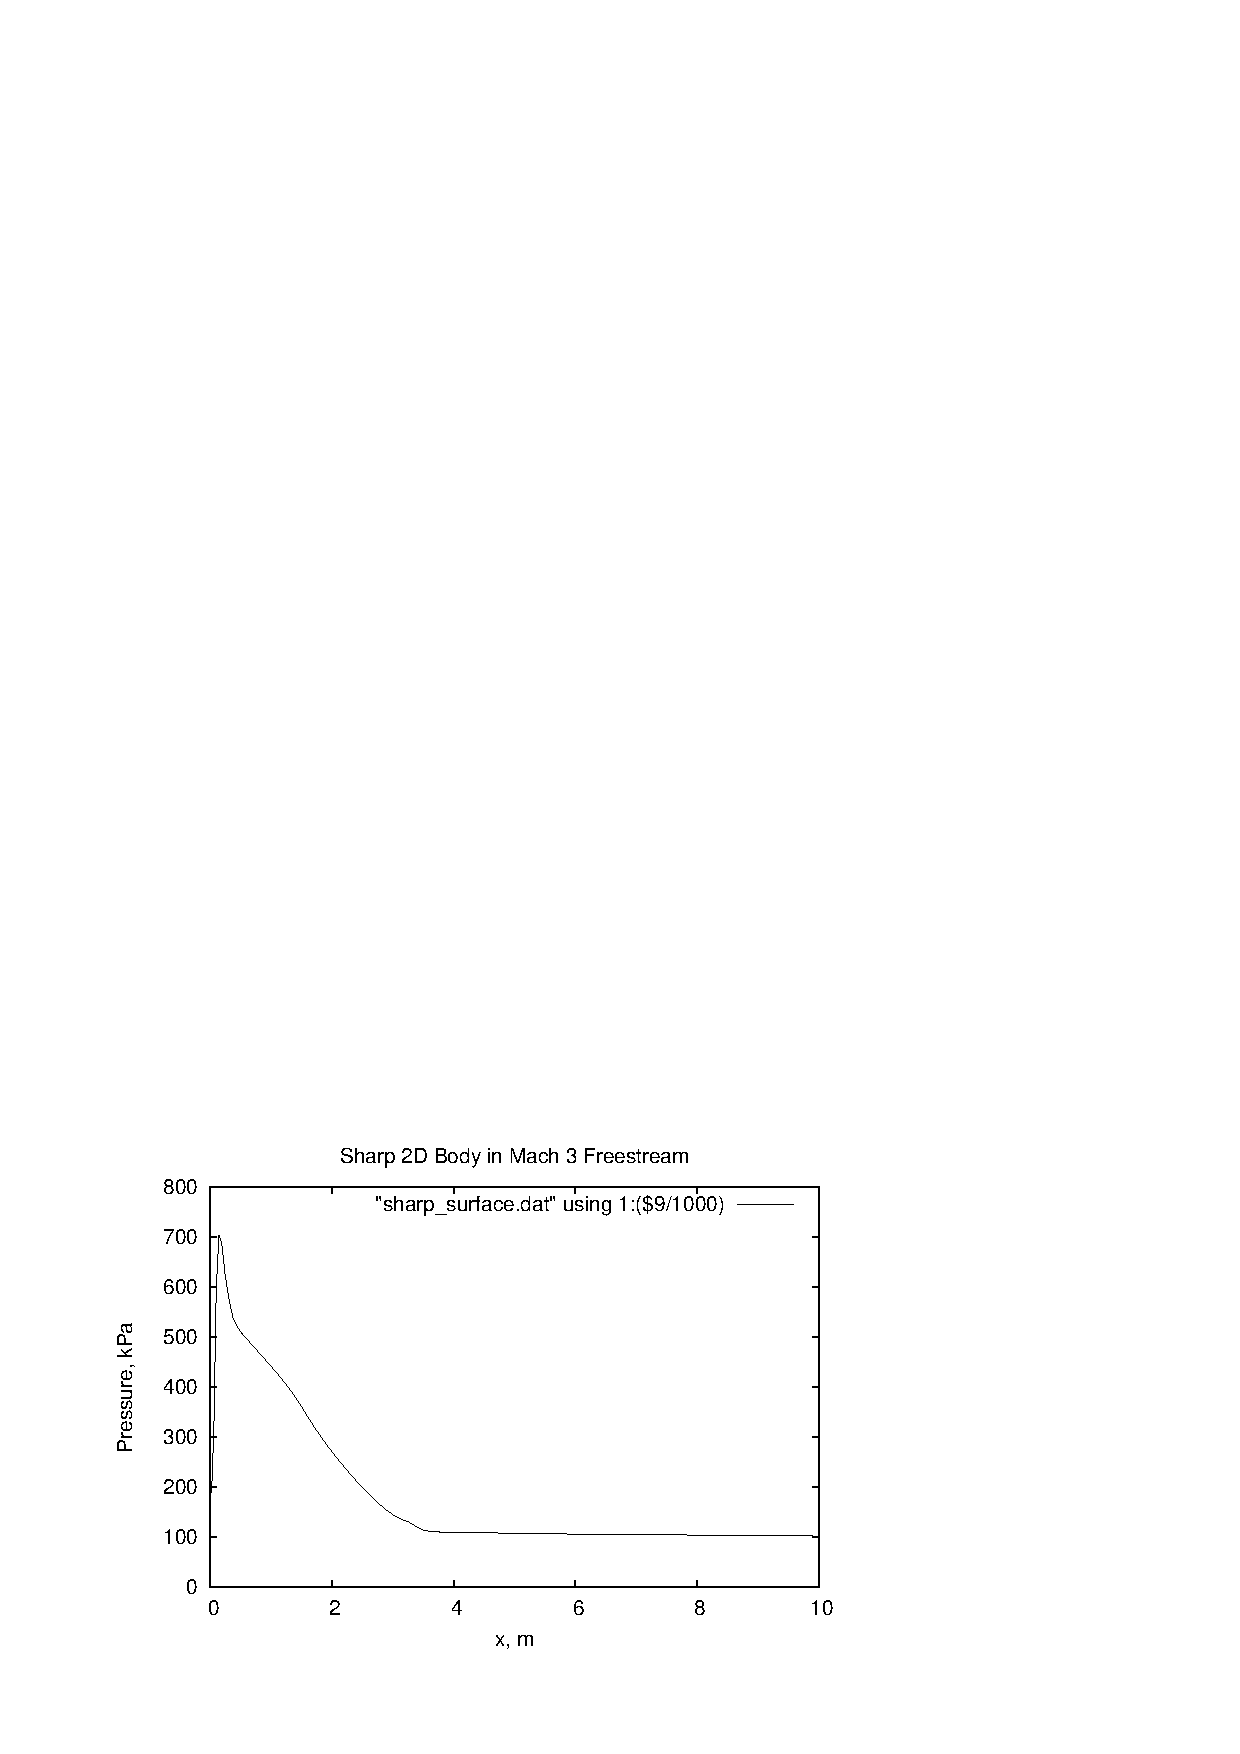
\includegraphics[width=12cm, viewport=55 49 401 292]{../2D/sharp/sharp_surface_p.pdf}
\end{center}
\caption{Pressure data along the body surface.}
\label{sharp-surface-pressure-fig}
\end{figure}

\medskip
The surface pressure (shown in Fig.~\ref{sharp-surface-pressure-fig})
has been extracted from the solution file by \texttt{e3post.py} by selecting the
south-most line of cells of block 1.
The pressure field (Fig.~\ref{sharp-p-fig}) shows the curved shock clearly.

\begin{figure}[htbp]
\begin{center}
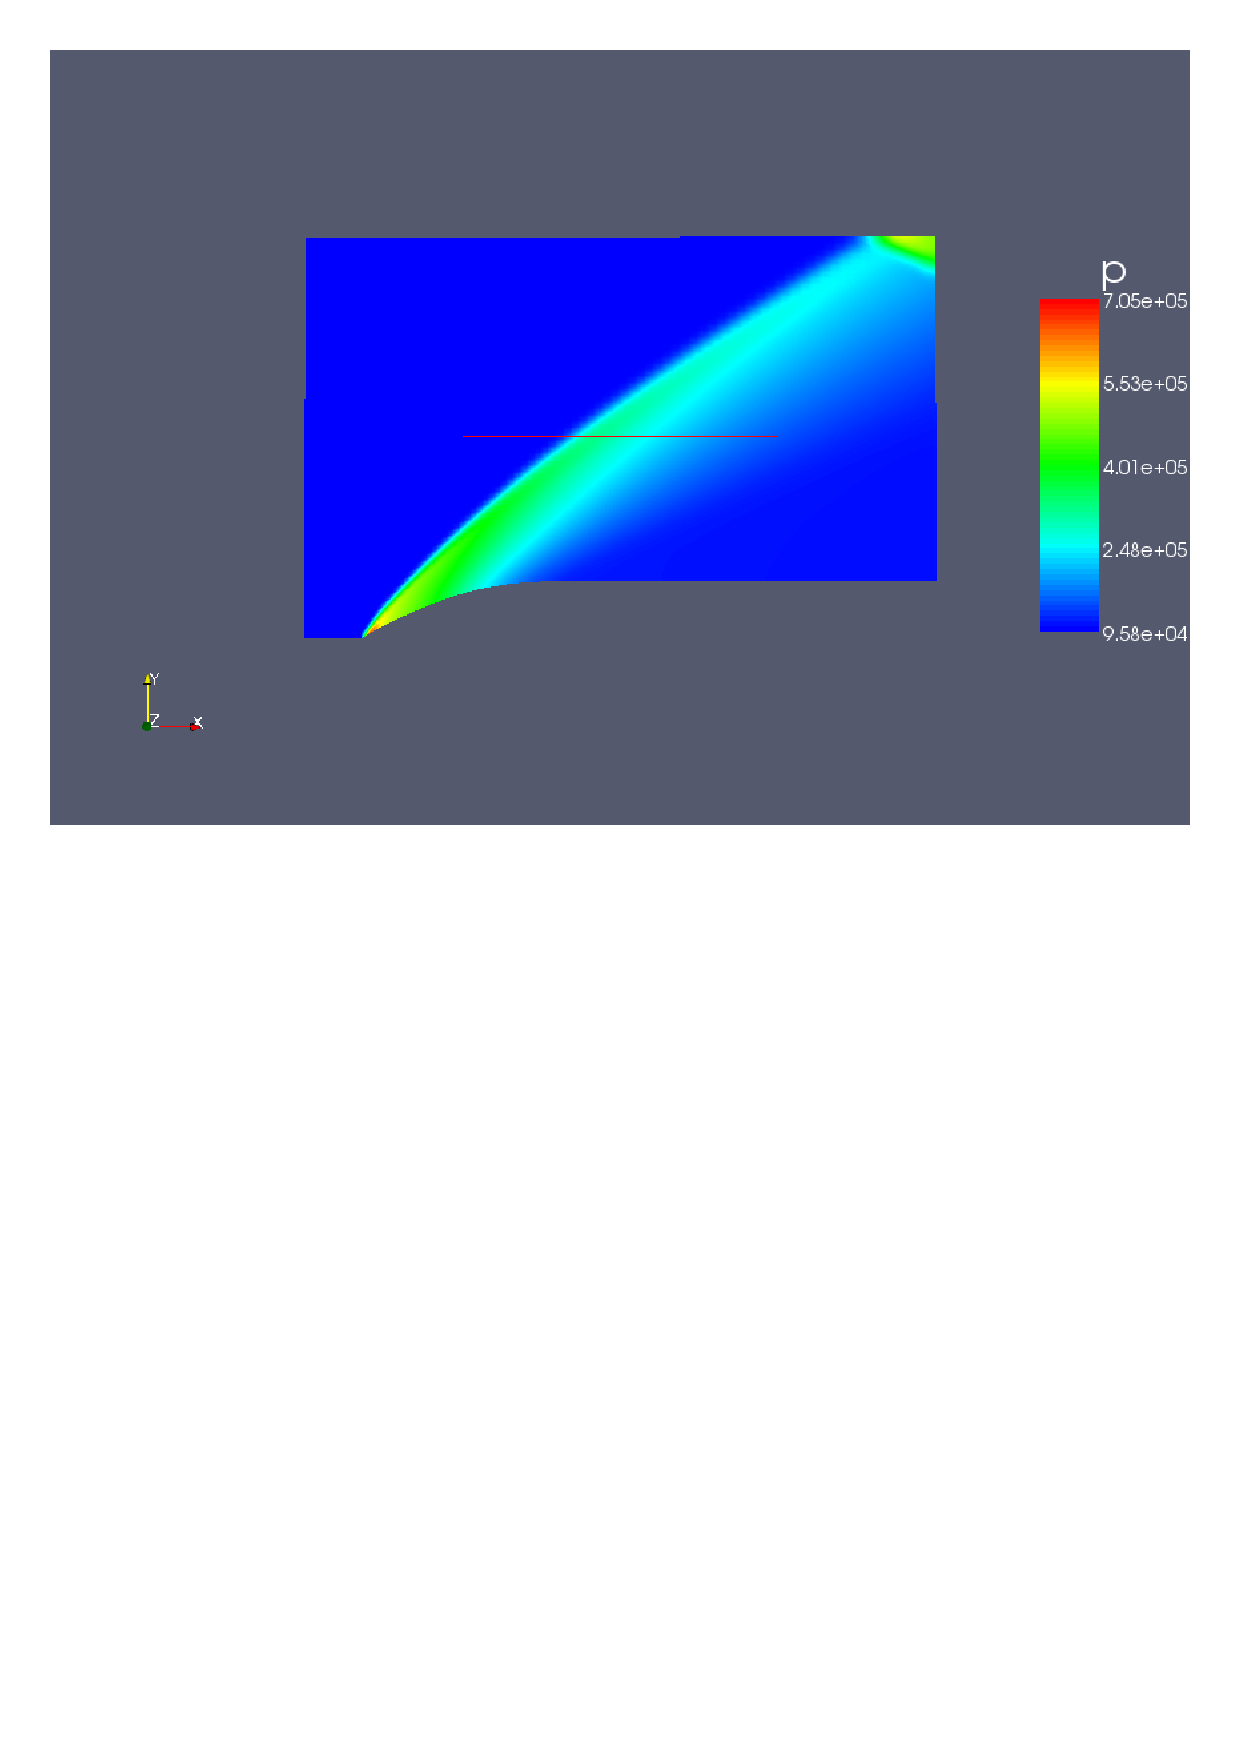
\includegraphics[width=\textwidth, viewport=24 446 570 818]{../2D/sharp/sharp_p.pdf}
\end{center}
\caption{The pressure field for flow over a sharp body.
    The data has been transformed from cells to points in Paraview.
    Note that the shock reflects from the upper boundary,
    which has a SLIP\_WALL boundary condition by default.}
\label{sharp-p-fig}
\end{figure}

\newpage

\subsection{Input script (.py)}
\index{univariate function!RobertsClusterFunction!example of use}
\index{geometric element!Spline!example of use}
\topbar
\lstinputlisting[language={}]{../2D/sharp/sharp.py}
\bottombar


\subsection{Shell scripts}
\label{sharp-sh-files}
\topbar
\lstinputlisting[language={}]{../2D/sharp/sharp_prep.sh}
\bottombar

\noindent
\topbar
\lstinputlisting[language={}]{../2D/sharp/sharp_run.sh}
\bottombar

\noindent
\topbar
\lstinputlisting[language={}]{../2D/sharp/sharp_post.sh}
\bottombar

\subsection{Notes}
\begin{itemize}
\item For mbcns2, this simulation reached a final time of 15\,ms in 1801 steps and,
  on a Pentium-M 1.73\,Ghz system, taking 2\,min, 48\,s of CPU time.
\item For Eilmer3, this simulation required 5\,min, 22\,sec on a single core of 
  a Pentium 1.6\,GHz processor.
  It reached the same time of 15\,ms in 1838 steps.
  As of September 2008, we clearly have some optimisation to do.
\end{itemize}
